\documentclass[12pt,a4paper,Flow]{report}
\usepackage[left=2.8cm,right=2.8cm,top=2.5cm,bottom=2cm]{geometry}
\usepackage[BoldFont]{xeCJK}
\usepackage{xcolor}
\usepackage{graphicx}
\usepackage{colortbl}
\usepackage{float}
\usepackage{indentfirst}
\usepackage{fancyhdr}
\usepackage[toc,header,title]{appendix}
\usepackage{listings}
\usepackage{tikz}
\defaultfontfeatures{Mapping=tex-text}
\definecolor{llgray}{rgb}{0.9,0.9,0.9}
\lstloadlanguages{[ansi]c}
\lstset{
  language=python,tabsize=4,keepspaces=true,
  xleftmargin=2em,xrightmargin=2em,aboveskip=1em,
  frame=none,
  commentstyle=\color{red}\itshape, % blue comments
  keywordstyle=\color{blue}\bfseries,
  backgroundcolor=\color{llgray},
  breakindent=22pt,
  numbers=left,stepnumber=1,numberstyle=\tiny,
  basicstyle=\footnotesize,
  showspaces=false,
  showstringspaces=false, % show explicit string spaces
  flexiblecolumns=false,%true,
  breaklines=true,breakautoindent=true,breakindent=4em,
  escapeinside={/*@}{@*/}
}
\usepackage[a4paper,CJKbookmarks,bookmarks=true,bookmarksopen=true]{hyperref}
\hypersetup{
  pdftitle={},
  pdfauthor={Wang Pei},
  pdfkeywords={},
  bookmarksnumbered,
  breaklinks=true,
  pdfview=FitV,       % Or try pdfstartview={FitV}, This lead to uncorre
  urlcolor=cyan,
  colorlinks=true,
  citecolor=magenta,          %citeref's color
  linkcolor=blue,
}
\usepackage{titlesec}
\titleformat{\chapter}{\centering\huge}{\textbf{第}\thechapter{} \textbf{章}}{1em}{\textbf}
\renewcommand\contentsname{目录}
\renewcommand{\appendixpagename}{附录}
\renewcommand{\appendixname}{附录}
\setmainfont{DejaVu Sans}
\setCJKmainfont[BoldFont=WenQuanYi Micro Hei]{SimSun}

\begin{document}
\title{\textbf{编译实习——minic编译器\\项目文档}}
\author{张番栋 00848180\\刘澜涛 00848200\\王 沛 00848205}
\date{}
\maketitle
\tableofcontents
\newpage
\chapter{实习内容}
实习的内容是以C语言编写一个以C语言子集(称为MiniC)为源程序,目标机为UniCore2体系结构的编译器。报告后面的篇幅中,均称实习中编写的编译器为minicc。MiniC的语法与C语言基本相同,比较重要的区别是不支持除法、浮点计算、多重指针和高维数组。\\
\indent 实习对minicc的基本要求是,可以对给定的源程序进行语法和语义上的正确性检查并能够输出正确的汇编程序代码,最终与体系结构实习所完成的模拟器协同工作。这一过程需要的预处理器、库以及二进制工具由外部提供。
\chapter{编译器前端}
minicc前端的任务有
\begin{enumerate}
\item 针对源程序进行词法、语法分析。
\item 在语法分析的过程中构建抽象语法树、建立符号表。
\item 针对语法树进行语义检查,包括类型检查与左值存在性检查。
\item 生成中间代码。
\end{enumerate}
下面对各项工作进行详细说明。
\newpage
\section{词法、语法分析}
minic的词法和语法分析部分代码由flex和bison辅助生成。\\
\indent 就词法分析而言,由于MiniC的文法并没有对源程序中字符、字符串的形式做规定,因此在实现时,我们只支持了最普通的一种,十六进制形式的字符和字符串常量并不被词法分析过程接受。\\
\indent 语法分析方面,我们对原始的MiniC文法进行了一定修改,使其支持悬空if控制流。另外通过规定运算符优先级和结合性的方式避免的文法规约时的二义性。
\section{构建抽象语法树}
处于简化数据结构的考虑,在语法分析的过程中仅对计算语句构建抽象语法树。控制流的实现在进行文法规约时同步处理,这一点在之后还会详细说明。\\
\indent minic语法总只有一元和二元运算符,因此将语法树定义为二叉结构。源程序中一个表达式对应一棵语法树,语法树的叶节点根据词法分析过程的返回信息生成,具体类型包括三种:整型常量、字符串常量和标识符。
\subsection{常量处理}
根据C语言标准,源程序中出现的字符常量全部视为整型常量,因此语法树中没有表示字符常量的结构。\\
\indent 对于标识符,语法树中会存储它的名字字符串,以便在符号表中查询。\\
比较特别的是对字符串常量的处理。在C语言中,字符串常量的生存期是整个程序运行期间,程序中对字符串常量的引用基本与全局变量相同。因此在构建语法树时,会将字符串常量视为类型为字符型指针的标识符。标识符名即为字符串在汇编代码中的标号。关于这一点,在构建符号表时也需要做一些特殊处理。\\
\subsection{函数参数}
在语法树的中间节点中,函数调用比较特殊。在我们的实现中,函数调用被视为一个二元操作,左操作数为函数标识符,右操作数为参数列表。这里的列表概念引自函数式语言,是多个元素的有序集合。为了在语法树中支持这种概念,我们引入Arglist这种运算。这种运算的操作数为一棵普通语法树的根,代表一个参数;右操作数是根据参数数量可以是空,也可以是另一个以Arglist运算为根的语法树。以这种递归式的结构就可以支持任何数量的参数列表。
\subsection{大立即数}
另一种比较特殊的结构是大立即数。minicc的目标机是UniCore2体系结构,而该体系结构的指令系统不支持超过9bit的立即数作为操作数,因此对于源程序中出现的较大的立即数不能简单视为常量。为了在这方面有所体现,在构建语法树时引入了一种新的运算,称之为BigImm,用于表示大立即数的产生。关于大立即数的产生算法,在生成机器指令时还会详细描述。
\subsection{样例}
下面给出一个表达式生成语法树的结果示例:
\begin{center}
  v1 = v2 * foo(c, v3) - 1 + *p;\\
  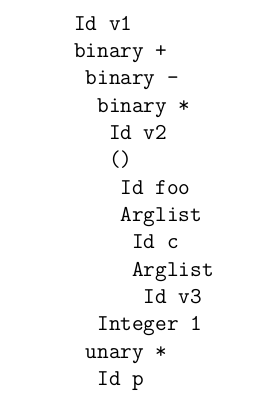
\includegraphics[width=0.4\textwidth]{ast-ex.png}
\end{center}
\section{符号表}
符号表用于存放源程序中与标识符有关的信息,包括标识符名,标识符类型,标识符属性(是否为extern)等。
\subsection{组织方式}
考虑到整个编译过程中的需要经常对符号表进行查询,所以我们以散列的方式对符号表进行组织。散列函数采用Unix经典的ELFHash,散列方式为开散列。符号表的构建在语法分析的同时进行。\\
\indent minic文法支持全局变量和单源文件多函数定义,因此符号表还需要存储与变量作用域有关的信息。我们的处理办法是开辟多个符号表,包括一个全局符号表和多个局部符号表。全局符号表存储全局变量和函数信息;每一个局部符号表对应一个函数,存储函数的局部变量和参数信息等。在对符号表进行查询时,需要首先在当前函数的局部符号表中进行查询,如果查询失败则再在全局符号表中进行查询。
\subsection{构建过程}
现在开始解释构建的详细过程。minic的与变量声明有关的文法如下:
\begin{verbatim}
declaration : modifier type_name var_list ";";
var_list : var_list "," var_item
         | var_item
         ;
\end{verbatim}
可以看到,在词法分析过程中遇到标识符时,并不能立刻得知其类型,需要再经过若干步规约才能得到一个声明序列中所有标识符的基类型,如下面的声明语句:
\begin{lstlisting}[language=c]
  int a, *b, c;
\end{lstlisting}
文法规约的顺序是自右向左,因此在分析到变量名时,变量类型还未归约,因此无法确定变量名的类型。解决的办法是开辟缓冲区对标识符进行暂存,待得到足够信息后再对符号表相应位置进行回填。\\
\indent 另一个比较重要的问题是对字符串常量的处理。之前已经提到,字符串常量在汇编代码中的出现方式与全局变量相似,因此为了方便处理,为每个字符串常量生成一个伪标识符。伪标识符以字符“.”开头,以便区分。
\section{语义检查}
语义检查主要分两部分:类型检查和左值存在性检查。
\subsection{类型检查}
\indent 类型检查的进行基于之前生成的语法树。检查的过程是一个递归的过程:先检查左右子树,得到左右子树的类型,然后根据当前节点的运算类型以及节点左右子树的数据类型在这期间对运算符和运算数的相容性进行检查,并计算当前节点的数据类型,也就是进行隐式类型转换。隐式类型转换的规则与[ANSI]C语言标准完全一致。如果出现类型不相容的情况,则给当前节点赋以Typeerror类型。当对整颗语法树检查完毕后,根据根节点即可得知该语法树对应的表达式中是否有语义错误,同时也得到了所有中间结果的数据类型。
\subsection{左值存在问题}
左值的存在性检查同类型检查在同一过程中进行。根据C语言语义,在进行赋值(=)操作时,要求左操作数拥有左值;在进行引用(\&)操作时,要求操作书拥有左值。拥有左值的变量有以下几种:
\begin{enumerate}
\item 标识符(因字符串常量引入的伪标识符除外)。
\item 解除引用运算(*)得到的结果。
\item 下标运算([])得到的结果。
\end{enumerate}
因此,左值检查的时机是赋值和引用运算,只有被检查的操作数是由上述运算产生时才可通过检查。
\section{中间代码生成}
minicc的中间代码只有一种,形式为间接三元式。一般而言,典型的中间代码形式有三元式和四元式两种。这里我们采取间接三元式是为了简化符号表操作,因为四元式需要引入众多临时变量。另外之前已经提到,我们的语法树无法表示控制流。如果采用四元式作为中间代码,那么在实现控制流时就比较繁琐,因为四元式不利于代码顺序的调整。\\
\indent 中间代码生成的结果基本是线性化的抽象语法树,下面给出根据之前的样例语法树生成的三元式序列。
\begin{verbatim}
(0) Arglist c 
(1) Arglist v3 
(2) () foo 
(3) binary * v2 (2) 
(4) binary - (3) 1 
(5) unary * p 
(6) binary + (4) (5) 
(7) = v1 (6) 
\end{verbatim}
三元式的第一部分为运算符,第二和第三部分为运算数。Arglist表示参数传递的操作。
\indent 在从语法树向三元式转化的过程中,有几个比较重要的问题需要解决。
\subsection{逻辑运算的短路}
第一个问题是逻辑运算的短路问题。根据C语言标准,逻辑运算需要是懒惰的,即在规定的求值顺序下,一旦逻辑表达式的真假可以被确定,则立即停止对表达式剩余部分的求值。要实现这一点,必须在逻辑表达式所对应的三元式中增加额外的跳转判断和跳转代码。\\
\indent 我们采取的解决方案是经典的拉链回填技术,即为每个逻辑表达式维护两个跳转地址链,链中存放需要回填跳转目标的三元式标号。因为在生成逻辑表达式子式对应的三元式,还不知道跳转目标地址,因此需要在链中暂存,至整个表达式分析完毕后再将目标地址回填。下面是一个样例:
\begin{lstlisting}[language=c]
  int foo(char * a, int x);
  int main()
  {
    int a, b, x;
    char * p;
    if(a > 1 || foo(p, x))
    b = 1;
    else
    b = 0;
    return 0;
  }
\end{lstlisting}
对应的三元式序列为
\begin{verbatim}
(2) > a 1 
(3) TrueJump (2) (0) 
(4) UncondJump (5) 
(5) Arglist p 
(6) Arglist x 
(7) () foo 
(8) TrueJump (7) (0) 
(9) UncondJump (1) 
(0) = b 1 
(10) UncondJump (11) 
(1) = b 0 
(11) Return 0 
\end{verbatim}
\subsection{逻辑值与算数值之间的转化}
C语言不区分逻辑值和算数值,因此像下面这样的代码是被允许的。
\begin{lstlisting}[language=c]
  int a, b, c;
  // ...
  a = (b < c || a < c) + 1;
\end{lstlisting}
在上面这种情况中,需要对逻辑表达式的结果进行暂存,然后令其参与后续运算。然而在大部分情况下,对于大多数体系结构而言,逻辑表达式的中间结果是不需要暂存的。如何处理这个问题就成了一个难点。这个问题和第一个问题结合在一起时,处理的难度就更大了。\\
\indent 要解决这个问题,需要在表示三元式的数据结构中增加一个域,用于表示当前结果是逻辑值还是算数值。如果在分析语法树某个节点时发现当前运算需要算数值作为操作数,但子树的根节点类型为逻辑值,则需要额外产生算数值的工作。由于三元式中没有显式的临时变量,因此只能引入一种新的操作来表示临时变量。上面表达式翻译成三元式序列的结果是
\begin{verbatim}
(0) < b c 
(1) TrueJump (0) (7) 
(2) UncondJump (3) 
(3) < a c 
(4) TrueJump (3) (7) 
(5) UncondJump (9) 
(6) Temp 
(7) = (6) 1 
(8) UncondJump (10) 
(9) = (6) 0 
(10) binary + (6) 1 
(11) = a (10) 
(12) Return 0 
\end{verbatim}
\subsection{三元式的组织}
我们采用三元式的原因之一,就是三元式利于调度。但是在实现具体的调度机制还是需要一些比较繁复的工作。
比如在实现for循环时,
\begin{lstlisting}
  for_stmt :
  FOR "(" expression ";" expression ";" expression ")" statement ;
\end{lstlisting}
表达式的规约顺序与最终三元式应该的顺序相差甚远。所以当语法分析到达这一步时,需要做一些调整工作。其他控制流的情况类似。
\chapter{编译器后端}
minic后端的任务有:
\begin{enumerate}
\item 根据中间代码进行数据流分析:划分基本块,判断变量的活跃周期。
\item 根据数据流分析的结果进行寄存器分配。
\item 生成目标代码
\end{enumerate}
\section{数据流分析}

\section{寄存器分配}
\subsection{图染色算法}
minic采用图染色法进行寄存器分配。算法流程是
\begin{enumerate}
\item 根据变量的活跃信息构造干涉图。为提高效率,图的结构有两种:三角相邻矩阵和邻接表,它们适用与不同的操作。
\item 搜索干涉图中度数小于可用寄存器数的节点,将其从图中删除并压栈。如果图中已经不存在任何节点,算法转4。如果途中不存在这样的节点,转3。
\item 根据一定策略,将途中某个节点抛出(spill),即将其标记为存储在栈中,并从图中删除。之后算法转2。
\item 从将栈中的节点弹出,分配颜色。
\end{enumerate}
上面算法中删除节点的操作利用相邻矩阵完成更搞笑,而分配颜色的操作利用邻接表完成更高效。算法主体如下:
\begin{lstlisting}[language=c]
  while(left > 0)
  {
    int spill = 1;
    /* igmatrix is the adjacent matrix of the interfer graph */
    get_degree((const char **)igmatrix, n, elem);
    /* sort nodes by degree */
    qsort(elem, n, sizeof(isort_elem), isort_elem_cmp);
    for(i = n - 1; i >= 0; --i)
    {
      if(allocated[elem[i].val])     /* i already allocated */
      continue;
      if(elem[i].key < max_reg)
      {
        /* i can be placed in a reg */
        stack[top++] = elem[i].val;     
        allocated[elem[i].val] = 1;
        delete_node(igmatrix, n, i);
        --left;
        spill = 0;
      }
    }
    if(spill)
    {
      for(i = 0; i < n; ++i)
      {
        if(allocated[elem[i].val])
        continue;
        else /* spill the var having the max degree */
        {
          delete_node(igmatrix, n, elem[i].val);
          (ret.result)[elem[i].val] = -1;
          allocated[elem[i].val] = 1;
          --left;
          break;
        }
      }
    }
  }
\end{lstlisting}
\subsection{抛出(spill)策略}
算法中的抛出(spill)策略比较简单,每次都选择产生干涉最多的变量进行抛出。由于UniCore2体系结构是通用寄存器结构,寄存器数目较多,所以即使是这样简单的寄存器分配策略也可以有很好的效果。
\section{机器码生成}
\subsection{大立即数产生算法}
UniCore2指令系统采用定长编码方式,指令长度为4个字节,因此无法直接使用较大的立即数作为指令操作数。与立即数有关的操作指令格式如下
\begin{center}
  \begin{tabular}{ccccc}
    8 bits & 5 bits & 5 bits & 5 bits & 9bits \\
    \hline
    operation \cellcolor{rgb:red,2;green,1;yellow,1}& rs\cellcolor{rgb:red,0;green,1;yellow,1} & rd\cellcolor{rgb:red,0;green,0;blue,1} & shift\_imm \cellcolor[gray]{.9}& imm\_operand \cellcolor{rgb:red,5;green,0;yellow,0}\\
    \hline
  \end{tabular}
\end{center}
对于这样格式的指令,第二个源操作是由9位的imm\_operand经过shift\_imm次循环右移得到的32位数。根据这个特点,所有立即数都可以通过将其拆分为若干部分,然后做或位运算得到。由于立即数编码中的0是无需产生的,因此可以跳过立即数中连续的0。\\
\indent 下面是描述minicc产生一般性的大立即数的算法的代码:
\begin{lstlisting}[language=c]
int lsb = 0; /* least significant bit position*/
int temp;
while(((target >> lsb) & 1) == 0)
  ++lsb;
/* rotate shift right by 32-lsb bits */
temp = (target >> lsb) & 0x1ff;
temp = (temp << lsb) | (temp >> (32 - lsb));

result = temp; /* move instruction */
lsb += 9;
while(lsb < 32)
{
  while(lsb < 32 && ((target >> lsb) & 1) == 0)
    ++lsb;
  if(lsb >= 32)
    break;
  temp = (target >> lsb) & 0x1ff;
  /* rotate shift right by 32-lsb bits */
  temp = temp << lsb | (temp >> (32 - lsb));
  result |= temp;               /* or instruction*/
  lsb += 9;
}
\end{lstlisting}
利用上面的算法,可以把立即数的产生控制在4条指令之内。\\
\indent 在判断大立即数时,将目标都视为无符号数。但在实际情况中,程序员用到绝对值较小的负数的情况还是较多的。对于-512到-1的立即数,可以通过一条not指令得到,无需采用上面算法。
\chapter{编译优化}
\section{指令调度}
之前已经提到,minic是需要与MiniSim模拟器协同工作的。因此,根据MiniSim的实现,可以通过一些指令调度策略来提高模拟的性能。\\
\indent MiniSim模拟五级流水结构,因此由于数据相关而产生的加载互锁是性能的一大瓶颈,我们的优化也主要针对这一情况。minicc通过将产生数据相关的load指令提前,可以有效减少加载互锁发生的次数。减少加载互锁的策略有:
\section{窥孔优化}
\section{优化效果}
\end{document}
